\documentclass[journal]{vgtc}                % final (journal style)
%\documentclass[review,journal]{vgtc}         % review (journal style)
%\documentclass[widereview]{vgtc}             % wide-spaced review
%\documentclass[preprint,journal]{vgtc}       % preprint (journal style)

%% Uncomment one of the lines above depending on where your paper is
%% in the conference process. ``review'' and ``widereview'' are for review
%% submission, ``preprint'' is for pre-publication, and the final version
%% doesn't use a specific qualifier.

%% Please use one of the ``review'' options in combination with the
%% assigned online id (see below) ONLY if your paper uses a double blind
%% review process. Some conferences, like IEEE Vis and InfoVis, have NOT
%% in the past.

%% Please use the ``preprint''  option when producing a preprint version
%% for sharing your article on an open access repository

%% Please note that the use of figures other than the optional teaser is not permitted on the first page
%% of the journal version.  Figures should begin on the second page and be
%% in CMYK or Grey scale format, otherwise, colour shifting may occur
%% during the printing process.  Papers submitted with figures other than the optional teaser on the
%% first page will be refused. Also, the teaser figure should only have the
%% width of the abstract as the template enforces it.

%% These few lines make a distinction between latex and pdflatex calls and they
%% bring in essential packages for graphics and font handling.
%% Note that due to the \DeclareGraphicsExtensions{} call it is no longer necessary
%% to provide the the path and extension of a graphics file:
%% 
\includegraphics{diamondrule} is completely sufficient.
%%
\ifpdf%                                % if we use pdflatex
  \pdfoutput=1\relax                   % create PDFs from pdfLaTeX
  \pdfcompresslevel=9                  % PDF Compression
  \pdfoptionpdfminorversion=7          % create PDF 1.7
  \ExecuteOptions{pdftex}
  \usepackage{graphicx}                % allow us to embed graphics files
  \DeclareGraphicsExtensions{.pdf,.png,.jpg,.jpeg} % for pdflatex we expect .pdf, .png, or .jpg files
\else%                                 % else we use pure latex
  \ExecuteOptions{dvips}
  \usepackage{graphicx}                % allow us to embed graphics files
  \DeclareGraphicsExtensions{.eps}     % for pure latex we expect eps files
\fi%

%% it is recomended to use ``\autoref{sec:bla}'' instead of ``Fig.~\ref{sec:bla}''
\graphicspath{{figures/}{pictures/}{images/}{./}} % where to search for the images

\usepackage{microtype}                 % use micro-typography (slightly more compact, better to read)
\PassOptionsToPackage{warn}{textcomp}  % to address font issues with \textrightarrow
\usepackage{textcomp}                  % use better special symbols
\usepackage{mathptmx}                  % use matching math font
\usepackage{times}                     % we use Times as the main font
\renewcommand*\ttdefault{txtt}         % a nicer typewriter font
\usepackage{cite}                      % needed to automatically sort the references
\usepackage{tabu}                      % only used for the table example
\usepackage{booktabs}                  % only used for the table example
\usepackage{amsfonts}
\usepackage{amsmath, algpseudocode}
\usepackage{algorithm, algorithmicx}
%% We encourage the use of mathptmx for consistent usage of times font
%% throughout the proceedings. However, if you encounter conflicts
%% with other math-related packages, you may want to disable it.

%% In preprint mode you may define your own headline. If not, the default IEEE copyright message will appear in preprint mode.
%\preprinttext{To appear in IEEE Transactions on Visualization and Computer Graphics.}

%% In preprint mode, this adds a link to the version of the paper on IEEEXplore
%% Uncomment this line when you produce a preprint version of the article 
%% after the article receives a DOI for the paper from IEEE
%\ieeedoi{xx.xxxx/TVCG.201x.xxxxxxx}

%% If you are submitting a paper to a conference for review with a double
%% blind reviewing process, please replace the value ``0'' below with your
%% OnlineID. Otherwise, you may safely leave it at ``0''.
\onlineid{0}

%% declare the category of your paper, only shown in review mode
\vgtccategory{Research}
%% please declare the paper type of your paper to help reviewers, only shown in review mode
%% choices:
%% * algorithm/technique
%% * application/design study
%% * evaluation
%% * system
%% * theory/model
\vgtcpapertype{please specify}


\newcommand{\stitle}[1]{\vspace*{0.4em}\noindent{\bf #1:\/}}
\newcommand{\sstitle}[1]{\vspace*{0.4em}\noindent{\bf #1\/.}}
\newcommand{\DQV}{\mathsf{QEVIS}}


\newcommand{\QM}[1]{{\color{blue}{#1}}}
%% Paper title.
\title{$\DQV$: Understanding and Diagnosing the Fine-grained Execution Process of Hive Query via Visualization}

%% This is how authors are specified in the journal style

%% indicate IEEE Member or Student Member in form indicated below
% \author{Roy G. Biv, Ed Grimley, \textit{Member, IEEE}, and Martha Stewart}
% \authorfooter{
% %% insert punctuation at end of each item
% \item
%  Roy G. Biv is with Starbucks Research. E-mail: roy.g.biv@aol.com.
% \item
%  Ed Grimley is with Grimley Widgets, Inc.. E-mail: ed.grimley@aol.com.
% \item
%  Martha Stewart is with Martha Stewart Enterprises at Microsoft
%  Research. E-mail: martha.stewart@marthastewart.com.
% }

%other entries to be set up for journal
% \shortauthortitle{Biv \MakeLowercase{\textit{et al.}}: Global Illumination for Fun and Profit}
%\shortauthortitle{Firstauthor \MakeLowercase{\textit{et al.}}: Paper Title}

%% Abstract section.
\abstract{
Understanding the query execution process of distributed databases is crucial to many real-world practices such as detecting query bottlenecks and improving system performance. However, analyzing distributed query execution is challenging due to a large number of parallel tasks and the complex dependencies among these tasks. Moreover, system statuses such as network and memory can also affect query execution in complicated ways. Existing techniques typically collect \textit{aggregate statistics} of system performance (e.g., CPU, memory, and disk I/O) or execution progress (e.g., operator duration), and thus cannot track \textit{fine-grained query execution process} at the atomic task level, which is key to reason the query behavior. To tackle this problem, we propose $\DQV$, a visual analytics system that supports understanding and diagnosing distributed query execution from multiple views in an interactive manner. We tailor-make an algorithm for temporal directed acyclic graph (TDAG) layout to visualize the overall structure and execution process of the query plan. A suite of novel visualization and interaction designs are introduced to analyze the tasks, data dependency, and relation between atom task execution and system performance metrics. We illustrate the effectiveness of our $\DQV$ with three real-world case studies (i.e., query optimization, system configuration and xxx) and interviews with domain experts.

%Understanding the query execution of distributed databases is crucial to many real-world practices such as detecting the query bottleneck and improving the system performance.  Such analysis is always challenging due to the large volume of tasks executed in parallel and the complex task dependencies. Moreover, the unpredicted system behaviors also affect the query execution case by case. Existing techniques usually evaluate the distributed query by the statistics of system performance (e.g., CPU, memory, and disk I/O) or execution metrics(e.g., operator duration), which lost the fine-grained information at the atom task level. To tackle this problem, we propose $\DQV$, a visual analytics system to interactively understand and diagnose the distributed query execution procedure from multiple levels. An optimized algorithm for the temporal directed acyclic graph(TDAG) layout is devised to show the overall query plan structure and execution process. A suite of novel visualization and interaction designs are integrated to estimate the correlation between the atom task trace and the system performance metrics.  We illustrate the effectiveness of our $\DQV$ with three case studies from real-world applications and interviews with domain experts.
} 
% end of abstract

%% Keywords that describe your work. Will show as 'Index Terms' in journal
%% please capitalize first letter and insert punctuation after last keyword
\keywords{Radiosity, global illumination, constant time}

%% ACM Computing Classification System (CCS). 
%% See <http://www.acm.org/class/1998/> for details.
%% The ``\CCScat'' command takes four arguments.

\CCScatlist{ % not used in journal version
 \CCScat{K.6.1}{Management of Computing and Information Systems}%
{Project and People Management}{Life Cycle};
 \CCScat{K.7.m}{The Computing Profession}{Miscellaneous}{Ethics}
}

%% A teaser figure can be included as follows
\teaser{
  \centering
  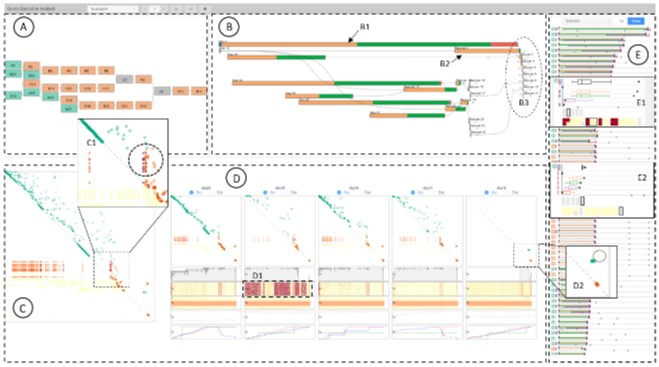
\includegraphics[width=\linewidth]{figures/teaser/teaser_mini3.jpg}
  \caption{In the Clouds: Vancouver from Cypress Mountain. Note that the teaser may not be wider than the abstract block.}
  \label{fig:teaser}
}

%% Uncomment below to disable the manuscript note
%\renewcommand{\manuscriptnotetxt}{}

%% Copyright space is enabled by default as required by guidelines.
%% It is disabled by the 'review' option or via the following command:
% \nocopyrightspace


\vgtcinsertpkg

%%%%%%%%%%%%%%%%%%%%%%%%%%%%%%%%%%%%%%%%%%%%%%%%%%%%%%%%%%%%%%%%
%%%%%%%%%%%%%%%%%%%%%% START OF THE PAPER %%%%%%%%%%%%%%%%%%%%%%
%%%%%%%%%%%%%%%%%%%%%%%%%%%%%%%%%%%%%%%%%%%%%%%%%%%%%%%%%%%%%%%%%

\begin{document}

%% The ``\maketitle'' command must be the first command after the
%% ``\begin{document}'' command. It prepares and prints the title block.

%% the only exception to this rule is the \firstsection command

\firstsection{Introduction}
\maketitle

The distributed database system is becoming increasingly pervasive due to the explosive growth of data in science, industrial and life.
Meanwhile, many management tools such as Hive, Flink and Vertical are developed to optimize the query, translate traditional query language to execution plan based on the map-reduce framework and dispatch multiple tasks to clusters to perform the data acquisition in parallel.

To maximally leverage the distributed systems, it is crucial for users to understand and evaluate how the query runs across the clusters. The frequently asked questions include "Where does the time go?", "What is the bottleneck of my query?", "Can we improve the performance of the specific query?".  Many research work devoted to evaluating and improving the performance of data analytics frameworks, but most of them try to reveal the performance by making high-level statistics about the correlated metrics collected from the accumulated logs or experiment conducted on benchmarks, which cannot be used for the understanding of the special case and provide the details answer for these questions. Specific methods which can look into the query execution process are required.

There are two challenges to facilitate the fine-grained inspection of query executions. 
\textbf{Non-transparent translation} makes it difficult for database users to inspect the query behaviors for a given abstract query. As shown by Figure**, the query issued by users is highly abstract which hides the detailed executed logic on a distributed system. The tools such as Hive can translate the query to a physical execution plan as shown by Figure~\ref{fig:exec_plan}. The execution plans have hundreds to thousands of lines of description, which is difficult for users to build a mental map for the overall execution plan. Existing work tries to bridge the gap between the execution logic and human perception by visualizing the execution plan as directed acyclic graph and allow users to interactively narrow down to any detailed operator as demand. However, the visualization of execution plan is always independent from the visualization of execution process. During the exploration, the users have to switch between multiple views which break the continuity of the plan-execution analysis.
\textbf{Unexpected behavior of distributed system} also increases he difficulty to understand the model execution process. For instance, the developer find that the same query execution plan run today may be different from that of yesterday. In general, four aspects are considered to affect the performance of clusters: CPU usage, memory usage, network IO and disk status. Existing work studies try to reveal how these metrics related to the system performance or quantify the impact and significance of these features. These studies are conducted based on the observed performance data from the experiment or logs collected from the production environment. One work inspired us is VQA which tries to linkage the resources status to query performance and resource usages. However, these work fail to provide the fine-grained execution traces for users to inspect the reasons of model behavior.

In this work, we develop a visual analytics system called DQSVis (Figure~\ref{fig:teaser}) for database users to monitor, understand and diagnose query behavior across the distributed system. The system can be run with three modes: 1) monitoring mode: the system runs with the query execution process, collects and visualizes the query status in real-time; 2) simulation mode: the system will replay the execution process with given simulation rate; 3) analysis mode: the system will directly show the final results for users to explore the final results. In the visualization component, we design a temporal DAG (directed acyclic graph) diagram to display the execution plan and execution process dynamically and seamlessly. To enable the scalable visual analysis of the large number of tasks executed on the computing nodes, we implement the compound trace diagram which integrates the point cloud form and progress bar form together to meet the different analysis requirements. The monitoring results are visualized in the monitoring view and linked with the other analysis views through a suit of flexible interactions. 


%% \section{Introduction} %for journal use above \firstsection{..} instead
\begin{itemize}
\item A framework to systematically analyze the query execution on distributed database by integrating three components: query analyzing component, machine monitoring component and analytic component.
\item Well-established visualization front-end to support the interactive investigating, comparing and diagnosing the query process. The system includes a set of novel designs for visualizing the temporal DAG and sequence group.
\item Case studies on the analysis of query process performed on the Hive platform.
\end{itemize}

\section{Related work}
\subsection{Query analysis}
Understanding the query behaviour and evaluting database performance has been studied for decades since the database management systems(DBMSs) have been found. Both database and visualization communities have proposed methods to analyze the performance and dignose the queires in automatic or manual way[][]. We give a brief introduction about the related works from the two following aspects: \textit{query logic structure} and \textit{query execution structure}, and refer the interested readers to~\cite{gathani2020debugging} for the systematic overview about the database query debug and performance analysis.

\emph{\textbf{Analyzing query structure}}. (SQL)Queries can be hard to read since they are always have a deep and nested structure. Many research works have been conducted to help the database users to quickly understand the quires. The most common method is to utlized visualization techniques to show the logic structure of operations[all]. For example, extended from previosu work, QueryVis utilzes the node-link diagrams to show the relationship between operators, the unambiguity is also proved in this paper. Other than the form of visualization, Gawade et al. proposed a method translate a query to Natural Language.  

\emph{\textbf{Analyzing query execution}}. 
After a query is issued by the database users, the query will be optimized and executed on the database platforms. Especially for the distributed database system, the query will be translated into the logic execution plans which is used to generating the physical tasks. Understanding the execution plans is important for users to expect the query performance. Many existing industrial sorfwares are developed to visualize the query execution process~\cite{tez-ui}. These softwares always utilize the gantt chart to show the progress and use Tree or directed acyclic graph(DAG) to show the relationship among the operators. VQA~\cite{simitsis2014vqa} displays the logic of query plan as a tree with the nodes indicating operators and the edge indicating the dataflow. Barcharts are inserted into the node to show the mertric of the operator(e.g., execution time, memory allocated). Perfopticon~\cite{moritz2015perfopticon} display the overall plan structure from two levels: fragment level and operator level. The system also allow users to observe the execution trace of fragment or operator across the workers.


\subsection{Visualization for sequence data}
Nowadays, large amount of sequence data are generated from a variety of applications such as health care~\cite{malik2015cohort, wongsuphasawat2011outflow}, social media~\cite{zhao2014fluxflow, law2018maqui}, and education~\cite{chen2015peakvizor, mu2019moocad, goulden2019ccvis, he2019vuc, chen2018viseq}.
As a special type of time-series data, event sequence record a series of discrete events in the time order of occurence~\cite{guo2020survey}. For the detail taxnomy about the time-series and event sequence visualization, we refer the readers to read the surveys~\cite{guo2020survey, silva2000visualization}. 

Sequence visualization are designed to reveal the information of event such as the event type, start time, end time and duration. Moreover, for the complex application requirement, various of the visualization tasks are proposed such visual summarization, prediction $\&$ recommendation, anormaly analysis and comparison. Existing visualization techniques can be classfied into five categories according to the form of visual representions, i.e., \emph{sankey-based visualization}, \emph{hierarchy-based visualizations}, \emph{chart-based visualizations}, \emph{timeline-based visualizations} and \emph{matrix-based visualizations}~\cite{guo2020survey}. 

\emph{\textbf{Hierarchy-based visualizations}}~\cite{gotz2019visual}, \emph{\textbf{sankey-based visualizations}} and \emph{\textbf{matrix-based visualizatios}} are always designed for displaying the sequence or sequence collection after modeling the them as special structures such as graph or tree.
For example, LifeFlow~\cite{wongsuphasawat2011lifeflow} utilizes the tree structure with a node presenting a group of events to summarize the sequences. Outflow~\cite{wongsuphasawat2011outflow} models the progression paths of sequences as directed acyclic graph with a node indicating a cluster of states, and then visualize the graph as sankey diagram~\cite{riehmann2005interactive}.  These methods always provide the highly abstract summarization for sequences and cannot directly reveal the pattern of specific individual sequence. Matrixwave~\cite{zhao2015matrixwave} uitilzes a sequence of matrix to show the connections between specific events, which can provide details connecting information of sequence. However, Matrixwave loss the detail temporal information and cannot be used to very large sequence collections. 

\emph{\textbf{Chart-based visualizations}} uses barchart, linechart or scatter plot to visualize the trend or distribution of events, which always works as assisting views to support the interactive explorations. For instance, barchart and linechart are always used to show the attributes distribution of sequences or temporal trends~\cite{gotz2019visual, cappers2017exploring}. Scatter plot can be used to show the overview of coarse-level overview of the sequence or sequence groups by project them to 2D canvas through dimension reduction algorithms or two specific attributes~\cite{wu2020visual, malik2016high, gotz2019visual}. Other than the  distribution of sequences, the scatter plot can also reveal the outliers. 

\emph{\textbf{Timeline-based visualizations}} are known as the most intuitive ways which demostrate the events in a time order. Gantt chart is a direct way to show the temporal information of event sequences, including the start time, end time and duration. Many industrial tools such as the TezViz uses gantt diagram to clearly demostrate progres of the operations. Lifeline~\cite{plaisant1996lifelines} use Gantt diagram to display the sequence as well as the events and each sequecne takes a single row. LiveGantt~\cite{jo2014livegantt} proposes an algorithm to visualize the scheduling events with better scalability. However, these methods cannot directly be used in our application since the dependencies of these sequences are ignored. Moreover, the gantt chart also suffers the series scalability problem when applied it to large sequence dataset and the abnormal sequence will be hidden without aligment.

\section{Background}\label{sec:background}

%The architecture and terms are introduced in this section to serve the as basis for the further discussions. 
%The figure~\ref{fig:architecture} demonstrates how a query is processed by a distributed query system. We use Hive based Hadoop architecture in this paper, and the analysis pipeline can be easily extended to other systems.


In this part, we introduce the query processing workflow of Hive (Hadoop-based) and related terminologies to facilitate further discussion. The query processing procedures of other distributed database systems are similar.  

\begin{figure}[t]
	\centering
	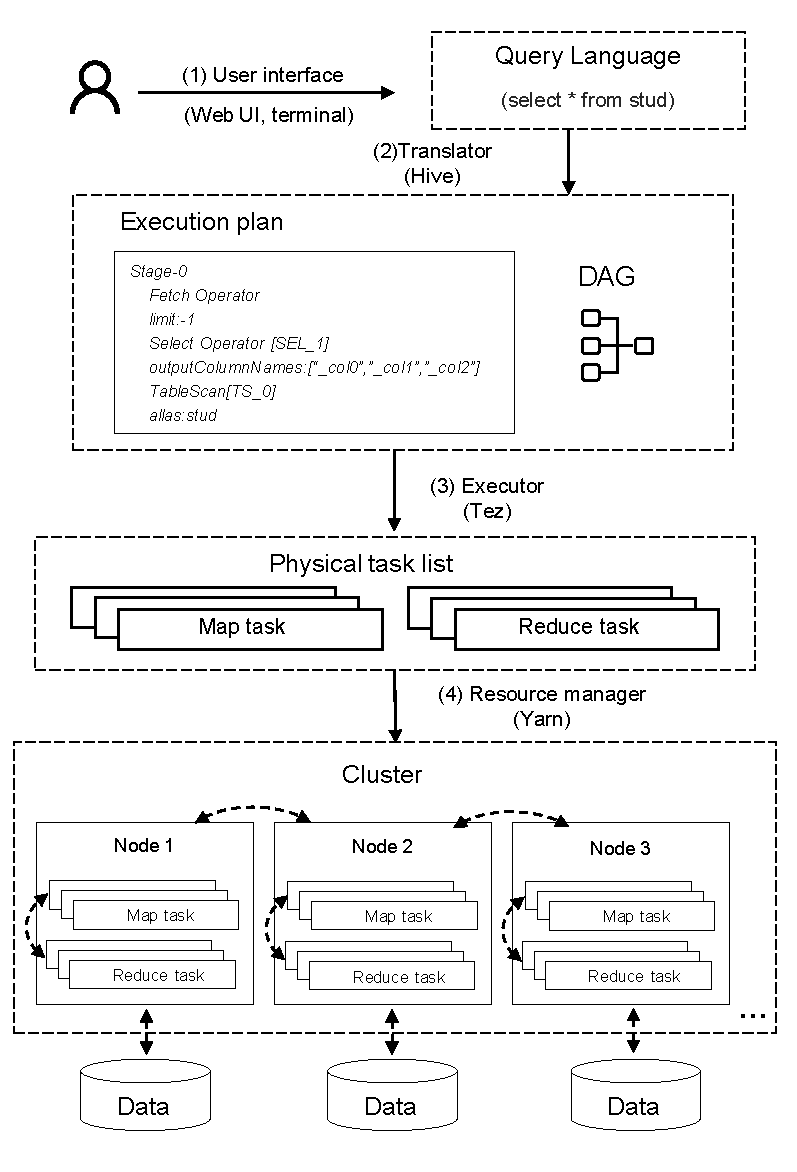
\includegraphics[width=0.42\textwidth]{figures/background/background.pdf}
	\vspace{-3mm}
	\caption{The query processing workflow of Hive (Hadoop 2.0).}
	\label{fig:architecture}
	\vspace{-3mm}
\end{figure}


As illustrated in Figure~\ref{fig:architecture}, query processing in Hive takes four steps. First, the user issues a query via some interface such as web-based UI or SQL terminal as shown in Figure~\ref{fig:architecture}-(1). Then, Hive uses a cost-based optimizer to optimize the query execution plan (e.g., select the best methods to conduct the scan operators, determine a good order for the join operators and choose the index to use) and obtains a logical execution plan as shown in Figure~\ref{fig:architecture}-(2). The logical exaction plan can contain hundreds of lines that describe the query execution process and will be executed by the computation engine (e.g., Tez). We can model the logical exaction plan as a Directed Acyclic Graph (DAG), in which each \textbf{vertex} corresponds to a sequence of logical operators (such as filter, aggregate and etc.) that conducts some sub-steps of the query. For Tez DAG, a vertex can be either a \textbf{map} vertex or a \textbf{reduce} vertex depending on it conducts map tasks or reduce tasks. The \textbf{edges} in a DAG are directed and model the data movement between vertices. For an edge, we call the source vertex \textbf{producer} vertex and the destination vertex \textbf{consumer} vertex. Note that a producer vertex may connect to multiple consumer vertices and a consumer vertex can take inputs from multiple producer vertices. 
 

%When user issues a query (shown as Figure~\ref{fig:architecture}(1)) through the interface such as a web-based user interface or SQL terminal. 
%Hive uses a cost-based optimizer to optimize the query such as determining the best methods for scan operators, join orders and aggregate operation, and then translate it as the logic execution plan shown as Figure~\ref{fig:architecture}(2). The logic exaction plan may contains hundreds of lines of description, which describes the execution process as a Directed Acyclic Graph(DAG) that can be processed by the executor(e.g., Tez). 

%A DAG is a collection of vertices and edges. Logically, a \textbf{vertex} consists of a sequence of logical operators(such as filter, aggregate, etc) which describes the execution of a part of the query. Further more, there are two types of vertices in the Tez DAG, \textbf{map} vertex and \textbf{reduce} vertex.  
%In the DAG,  the \textbf{edges} define the data movement between the adjacent vertices. We name of source vertex as the \textbf{producer} vertex and the target vertex as the \textbf{consumer} vertex. Noticed that a producer vertex may connect to multiple consumer vertices and a consumer vertex could be connected by multiple producer vertices.  

%With a given vertex, Tez further creates a set of atomic \textbf{tasks}(shown as Figure~\ref{fig:architecture}(3)). Then these tasks will be dispatched on the physical machines by Yarn, the resource manage tool of Hadoop2.0. A task takes a piece of data as input and execute all operators defined in the corresponding vertex. To ease the analysis of tasks, we define the sub-processes of a task as five steps. For a map task, the steps are \textit{Initialization}, \textit{Input}, \textit{Processor}, \textit{Sink}, \textit{Spill}. For a reduce task, the second step is \textit{Shuffle} instead. Moreover, the data read by a task could come from the local file or producer tasks.

%With the logical DAG, Tez generates the physical execution plan by spawning a set of atomic \textbf{tasks} for each vertex (as shown in Figure~\ref{fig:architecture}-(3)). Then these tasks will be dispatched on the physical machines by Yarn, the resource manage tool of Hadoop2.0. A task takes a piece of data as input and execute all operators defined in the corresponding vertex. To ease the analysis of tasks, we define the sub-processes of a task as five steps. For a map task, the steps are \textit{Initialization}, \textit{Input}, \textit{Processor}, \textit{Sink}, \textit{Spill}. For a reduce task, the second step is \textit{Shuffle} instead. Moreover, the data read by a task could come from the local file or producer tasks.


According to the logical DAG, Tez generates the physical execution plan by spawning a set of atomic \textbf{tasks} for each vertex (as shown in Figure~\ref{fig:architecture}-(3)). These tasks are then dispatched to the physical machines by Yarn as shown in Figure~\ref{fig:architecture}-(4), the resource manager of Hadoop2.0. Each task takes a piece of data as input and executes all the operators in its corresponding DAG vertex. To track the fine-grained execution process of the tasks, we decompose each task into five steps. For a map task, the steps are \textit{Initialize}, \textit{Input}, \textit{Process}, \textit{Sink}, \textit{Spill}. For a reduce task, the second step is \textit{Shuffle} instead of \textit{Input}. Note that the data read by a task could come from its local file or remote producer tasks.




\section{Design Goals and System Architecture}\label{sec:systemdesign}

In this part, we identify the design goals of $\DQV$ as a visualization system that supports fine-grained understanding of the query execution process and introduce its overall architecture.   


\subsection{Requirement Analysis}
%During one year of collaboration, we have closely collaborated with three experts in distributed database, who are also the co-authors of this paper.
%
%In the first month of the collaboration, we have held brainstorming to collect the most frequent raised questions when analyzing the distributed query system performance. Based the discussions with domain experts and review of existing literature, we have formulated the following design requirements.

In the $\DQV$ project, we collaborated closely with three experts in distributed database systems, who are also co-authors of this paper. In the first month of the project, we brainstormed to collect the most frequently raised questions when analyzing the performance of distributed query processing. Based on these discussions and by reviewing existing literature, we identified the following design requirements for $\DQV$.

%\begin{itemize}
%  \item[\textbf{R1}]\textbf{Understand the general query execution progress and query plan structure.} Before our collaboration, the domain experts have used profiling software (Tez  UI, etc) or visualization tools(Tableau, etc) to show the query progress as Gantt chart and query plan structure as directed graph. However, these two visualizations are always displayed in separated views which require users to switch their focus thus break the continuity of exploration.
%  \item[\textbf{R2}]\textbf{Understand the query process at the task level.}Tez task is the atomic level of executions because ny failure operation in the task will lead to the re-run of whole task. Understand the execution of single task can be helpful to identify the bottleneck of the whole query process. However, visualize the tasks is challenge. First, to visualize the tasks in traditional way(Gantt chart) need a very large rendering space. Multiple features such as the size of input/output data and the operators should be visualized for understanding the task. Moreover, the many to many relationship among the tasks also makes it difficult to design clear and \textbf{scaleble} visualization.
%  \item[\textbf{R3}]\textbf{Provide the visual insight to reason the behaviour and pattern of a specific task.}To solely visualize the tasks themselves are not enough to explain the specific pattern of tasks. Many performance of hardware resource such as the network status, hard disk waiting list is also related to the patterns. Such kinds of information should be vitalized effectively to assist the exploration of query executions. 
%  \item[\textbf{R4}]\textbf{ Support interactive exploration.} Other than the visualization designs, a flexible interaction should be implemented for users to navigate to any time range, vertex, task group or single task of interest. The linkage among the correlated visual elements are also should be considered om the design to coordinate the information.
%\end{itemize}


\begin{itemize}
	\item[\textbf{R1}]\textbf{Visualize the logical query plan and overall query execution progress.} Before our collaboration, the domain experts used profiling software (Tez  UI, etc) or visualization tools (Tableau, etc) to show the query plan as DAG and the query progress as Gantt chart. Although the two views help understanding query processing, the domain experts complained that they need to switch their focuses back and forth as the two views are separated, which breaks the continuity of exploration.
	
	\item[\textbf{R2}]\textbf{Understand the query process at the task level.}Tez task is the atomic level of executions because ny failure operation in the task will lead to the re-run of whole task. Understand the execution of single task can be helpful to identify the bottleneck of the whole query process. However, visualize the tasks is challenge. First, to visualize the tasks in traditional way(Gantt chart) need a very large rendering space. Multiple features such as the size of input/output data and the operators should be visualized for understanding the task. Moreover, the many to many relationship among the tasks also makes it difficult to design clear and \textbf{scaleble} visualization.
	\item[\textbf{R3}]\textbf{Provide the visual insight to reason the behaviour and pattern of a specific task.}To solely visualize the tasks themselves are not enough to explain the specific pattern of tasks. Many performance of hardware resource such as the network status, hard disk waiting list is also related to the patterns. Such kinds of information should be vitalized effectively to assist the exploration of query executions. 
	\item[\textbf{R4}]\textbf{ Support interactive exploration.} Other than the visualization designs, a flexible interaction should be implemented for users to navigate to any time range, vertex, task group or single task of interest. The linkage among the correlated visual elements are also should be considered om the design to coordinate the information.
\end{itemize}

\subsection{Task Analysis}
Guided by the aforementioned requirements, we discussed with the domain experts about the visualization form and distilled the following visualization tasks:

\begin{itemize}
  \item[\textbf{T1}]\textbf{Visualize the execution process and query plan structure effectively.} To guarantee the continuity of exploration(R1), the process and plan structure should be integrated into one visualization view. Several criteria should be considered such as the minimize usage of canvas, minimize the cross of links and provide clear topology structure.
  \item[\textbf{T2}]\textbf{Effectively visualize the information of tasks.} To facilitate the fine grained exploration of query execution(\textbf{R1}, \textbf{R2}), the information about the tasks should be visualized, including: the size of data processed by the task; the data-flow among the tasks; the temporal information of task(start the time, end time, duration, etc) and the corresponding sub-process. Moreover, the abnormal(tasks taking longer time) tasks and the specific execution trace should be easily observed.
  \item[\textbf{T3}]\textbf{Visualize the machine status.} Display the machine status such as network status, disk IO pending list, CPU usage and Memory Usage will be useful to investigate the characters of task, and reasoning the patterns of the query execution( \textbf{R3}). These performance metrics should be well linked with the specific patterns of tasks. 
  \item[\textbf{T4}]\textbf{Interaction and linkage.} System should provide the flexible interactions allowing users to switch the focus among the different point of interest, such as a specific time range, a vertex or a group of tasks(\textbf{R2}, \textbf{R3}, \textbf{R4}). For example, user may select a vertex and explore if the tasks in this vertex are CPU-bound or I/O-bound. This requires the visualization to show the related tasks when choosing a vertex and highlight the corresponding CPU usage and disk information simultaneously.


\end{itemize}


\subsection{System Architecture}
\begin{figure}[t]
	\centering
	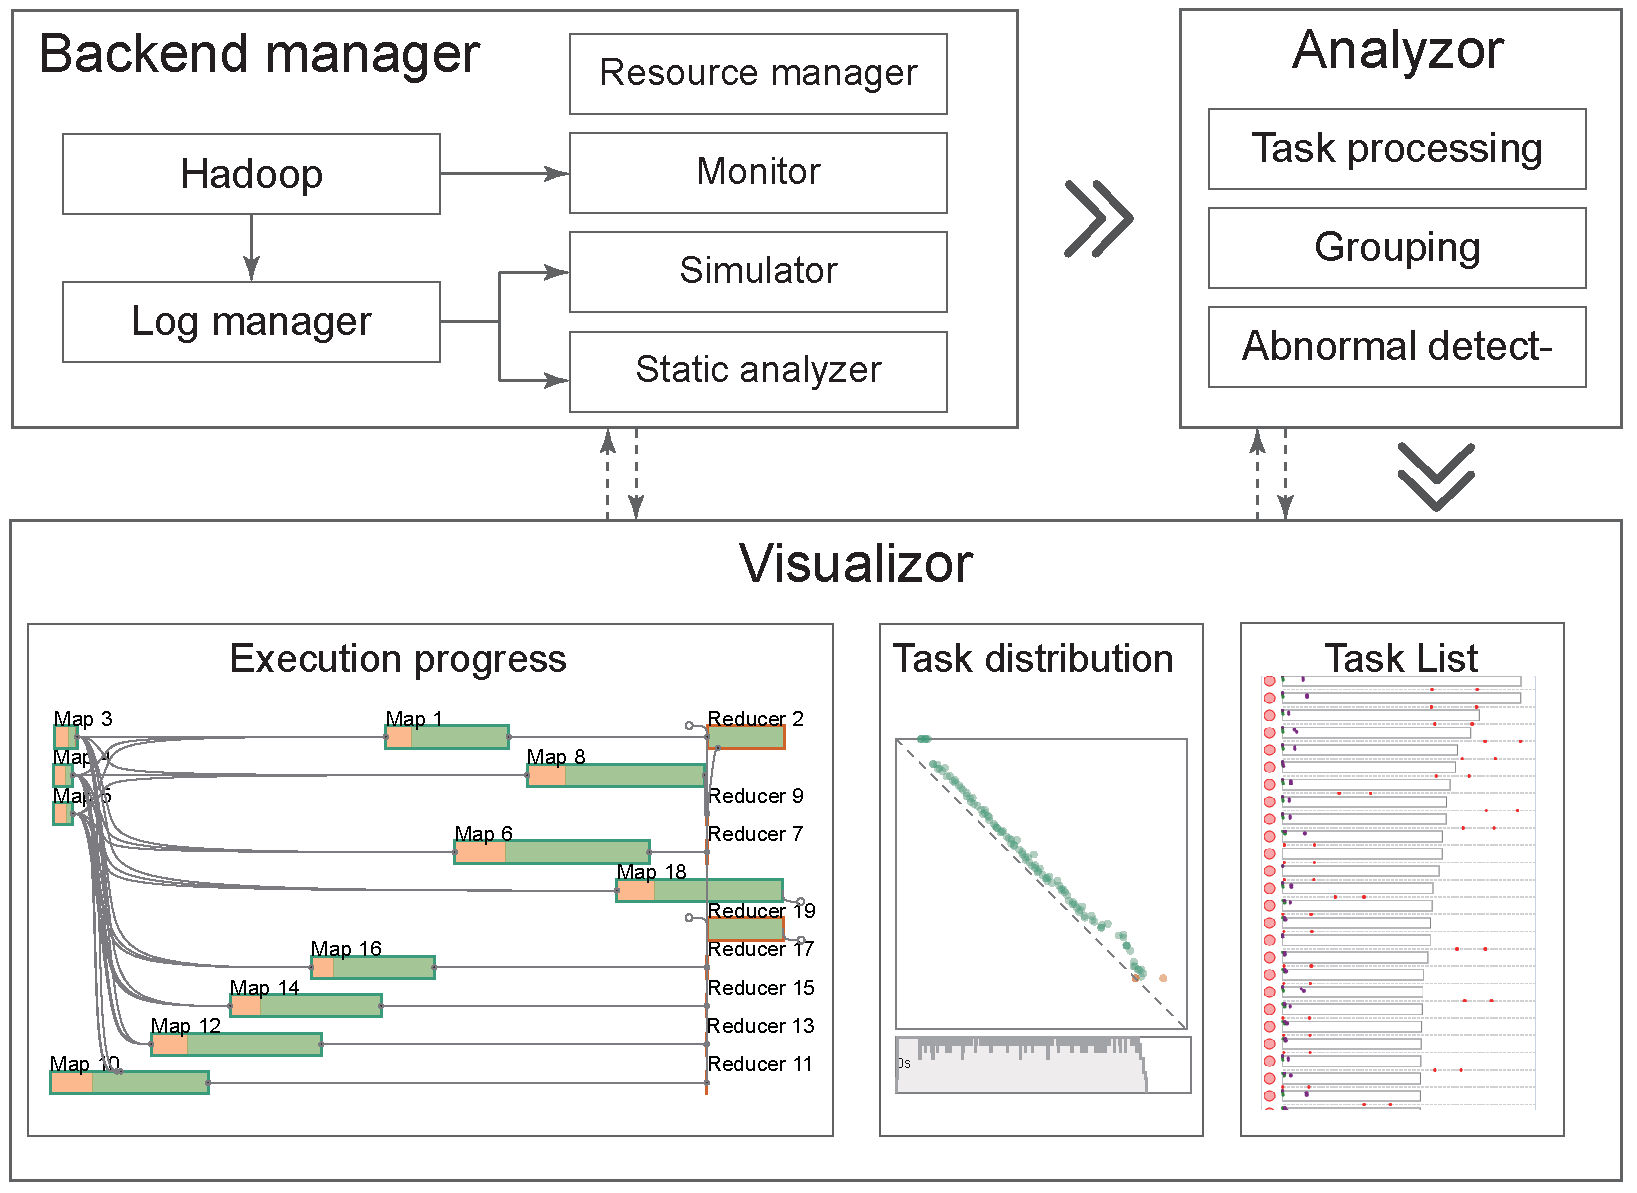
\includegraphics[width=0.45\textwidth]{figures/system/sysdesign.pdf}
	\vspace{-3mm}
	\caption{$\DQV$ system consists of three major components: backend manager, analyzer and visualizer.}
	\label{fig:sysdesign}
	\vspace{-3mm}
\end{figure}
We use build $\DQV$ based on Hadoop2.0 with \textbf{Hive} as query optimizer and \textbf{Tez} as the executor. As shown by Figure~\ref{fig:sysdesign}, $\DQV$ consists of three modules: backend manager, analyzer, and visualizer. 


The \textbf{Backend Manager} module performs the log processing and data fusion. Two categories of data are collected and fused: the execution data and the system performance data.
When collecting the execution data from Hadoop system, the Log Manager cleans and preprocesses the log files, extracts the important metrics and saves them as the local files.
Log analyzer directly takes these files as input and processes them as structured data for future processing.
Monitor module segments the data at the specific time range and output them with a given rate.
The simulator simulates the execution progress, allowing users to adjust the running speed and explore the dynamic query process.
Moreover, Resource Manager collect the system performance metrics and output them to the next processing stage.


The \textbf{Analyzer} fuses the execution data and system performance data by timestamps. The tasks will be grouped according to the vertex of the execution plan. The dataflow dependencies are recorded in this step. Moreover, Analyzor also performs the anomaly detection for the tasks in a group to enable the in-depth analysis.


The \textbf{Visualizor} module integrates coordinated views to support interactive exploration of query execution results and reasoning about the query behavior at multiple levels. The Execution Overview demonstrates the execution process at the vertex level. An algorithm for the temporal DAG is proposed to visualize the structure and procedure simultaneously. The task group view consists of two components: 1) task overview visualizes the temporal information and data dependencies of tasks executed on the same machine; 2) metrics component shows the corresponding machine performance metrics. The task list view provides more detailed information at the operator level, enabling the users to understand and compare the time usage of tasks. 


\section{Preprocess and data analysis}
\subsection{Data Collection}
As shown by figure~\ref{fig:sysdesign}, our analysis pipeline starts from the plan, log, and system performance data collection.

\stitle{Query plan parsing}
As shown in section~\ref{sec:background}, in Hive, an execution plan is described as a text file involving hundreds to thousands of lines of operations. We parse this file first and generate a directed acyclic graph with the node as the logic vertex and the edge as the data dependencies.

\stitle{Execution log and system performance processing}
Since the Hadoop execution logs are collected with the tedious system log, we locate the records of interest by detecting the keywords from the pre-defined keyword set and then parse these logs and extract the information.
Several important information is saved to the local file, including the task id, the logic vertices corresponding to the tasks, the temporal information(start time, duration) of tasks, the temporal information of steps in a task, etc. 

\subsection{Data Modeling}

\begin{figure}[t]
	\centering
	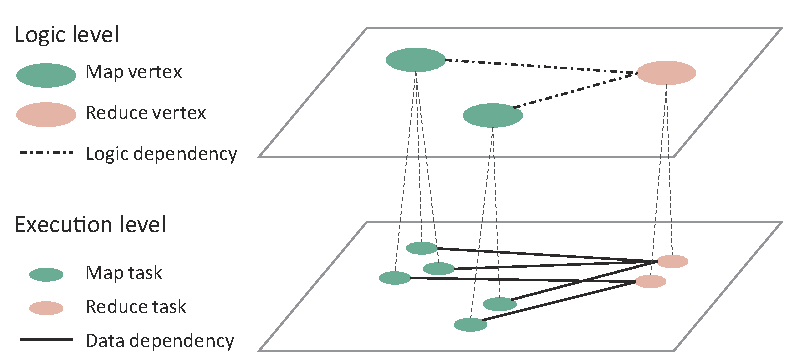
\includegraphics[width=0.42\textwidth]{figures/model/datamodel.pdf}
	\vspace{-3mm}
	\caption{Two-level temporal graph.}
	\label{fig:model}
	\vspace{-3mm}
\end{figure}

The data we collected from backend can be modeled as a temporal graph with two levels: the logic-level and execution-level, which is shown as the figure~\ref{fig:model}. 

As discussed in section~\ref{sec:background}, the logic level graph indicates the DAG extracted from the execution plan, denoted by $\mathbb{G}_L = (\mathbb{V}_L, \mathbb{D}_L)$, where $\mathbb{V}_L$ is the logic vertex set and the $\mathbb{D}_L$ is logic dependency set between the vertices. The execution-level graph denotes the $\mathbb{G}_E = (\mathbb{T}_E, \mathbb{D}_E)$, where $\mathbb{T}_E$ denotes the set of tasks executed by the the physical machines and $\mathbb{D}_E$ indicates the data dependency set between tasks. 
If a task $t \in \mathbb{T}_E$ is an physical instance of vertex $v \in \mathbb{V}_L$, we describe this relationship as the form $t \to v$. We also adopt the this description for the relationship between logic dependency $d_L \in \mathbb{D}_L$ and data dependency $d_E \in \mathbb{D}_E$ such as $d_e \to d_L$. Moreover, we use $P(v) = \{t|\forall t \to v\}$ to indicate all tasks which are the physical instances of $\mathbb{V}_L$. 
A map task $t$ has five steps indicating as an array: $S=<s_{init}, s_{input}, s_{proc}, s_{sink}, s_{spill}>$ and a reduce task have five steps $S=<s_{init}, s_{shuffle}, s_{proc}, s_{sink}, s_{spill}>$. Each step can be modeled by a pair of attributes $<st, d>$ which denotes the start time and durzation. Notice that the different steps of the same task may have overlap in time.

According to section~\ref{sec:background}, each task can be modeled as a sequence of attributes: $t:=<st, d, v, m, S_E>$, where $st$, $d$ and $v$ indicate the \textit{start time}, \textit{duration} and logic vertex of task $t$.  $m$ is the machine executes this task and $S_T$ is the corresponding steps. We use $t.attr$ to indicate the $attr$ of $t$.

The vertex can be modeled as triplet: $v:=<st, d, S_L>$. The start time of $v$ is $v.st=min(\{t.st|t \in P(v)\})$, the duration of vertex $e$ is $v.d=v.st+max(\{(v.st+v.d)|t \in P(v) \})$. The steps $S_L=$ $\{d_{init}, d_{input}, d_{proc}, d_{sink}, d_{spill}\}$ or $\{d_{init}, d_{shuffle}, d_{proc}, d_{sink}, d_{spill}\}$ according to the types, and with a given $v$, $d.attr = sum(\{s.attr| s\in S_L\})$ where $attr \in \{init, input, shuffle, proc, sink, spill\}$. 
% \section{Visualization design}
% \subsection{Query execution overview}
% \subsubsection{Execution plan view}
% \subsubsection{Execution progress view}
% \subsection{Task view}
% \subsection{System profiling visualization}
% \subsection{Linkage and interactions}

\section{Visualization design}
Following the data modeling, we present the web-based visual analytics system to support the interactive exploration with four coordinated views. The Execution progress demonstrates the overview about how the query plan are execute(\textbf{T1}), the Task distribution view shows the task distribution and the data dependencies. Integrated with the machine performance metrics, this view is also used for reason the specific patterns of tasks(\textbf{T2} and \textbf{T3}).  Task list provides the detailed information at the task level(\textbf{T2}).  At last, the interaction and linkage are introduced to support the multi-level explorations(\textbf{T4}).

\subsection{Query Progress View}


\begin{figure}[t]
	\centering
	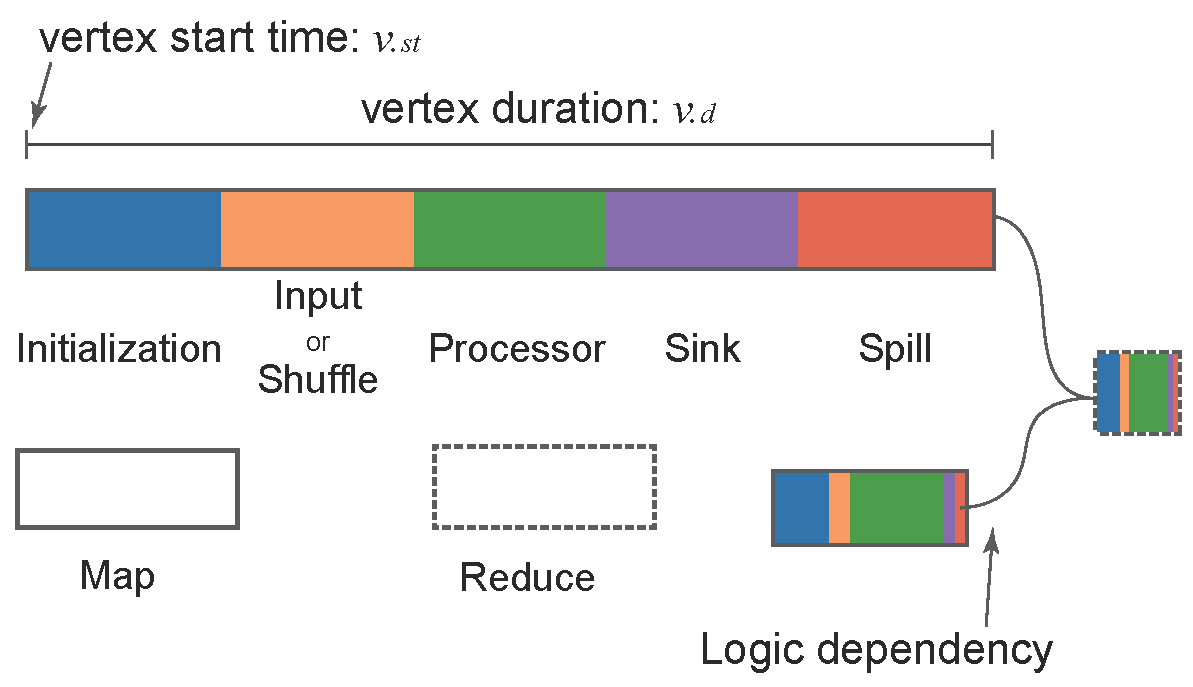
\includegraphics[width=0.40\textwidth]{figures/visualization/progressdesign.pdf}
	\vspace{-3mm}
	\caption{Visual encoding of logic vertex and dependency}
	\label{fig:progress}
	\vspace{-3mm}
\end{figure}


Query Progress View is developed to overview the overall progress of query execution and the logic dependencies. 
The commonly used methods to visualize the progress data is Gantt chart.

As shown by figure~\ref{fig:progress}, the x-axis indicates the timestamp. The rectangles with the same  height indicate the temporal information of logic vertices. Given a vertex $v$, the position of left sides indicates the start time $v.st$ and the duration of $v.d$ is encoded by the length of the rectangle. We use the color to encode the step and the stroke dash style to encode the type of vertex as shown by figure~\ref{fig:progress}.

%\begin{itemize}
%    \item Traditional method: Gantt diagram and design consideration 
%    \item Proposed algorithms, link processing
%    \item Alternative design
%        \begin{itemize}
%            \item Gantt(consider the vertical edge, large space, unclear structure)
%            \item New design loose(clear structure, large space)
%            \item New design compact(small space, unclear structure)
%        \end{itemize}
%\end{itemize}

% -Visual form of Gantt diagram
% -Our design consideration
% -Algorithms
% -Design alternatives
% --gantt(consider the vertical edge, large space, unclear structure)
% --new design loose(clear structure, large space)
% --new design compact(small space, unclear structure)
% --new design compact, edge processing(small space, clear structure)
\subsection{Task view}
\begin{itemize}
    \item Design consideration. Why gantt doesn't work(need very large space, difficult to show the data-flow link, difficult to show and select the abnormal cases)
    \item Our design
    \item Compare with design alternative (Gantt)
\end{itemize}


\subsection{Profiling view}
\begin{itemize}
    \item Our design consideration
    \item Design: Embedding task view to profiling view
    \item Design: Visualize the profiling results
\end{itemize}

\subsection{Interactions}
\begin{itemize}
    \item Multi-scale navigation
    \item Inner and inter linking
\end{itemize}

\section{Evaluation}
\subsection{Case study}
We demonstrate the effectiveness of $\DQV$ by analyzing several real world cases which are performed on the simulation mode. 

\subsubsection{Identify the bottleneck}
In this case study, we select a query case which runs longer than the expection. This case run ** seconds and is executed on an cluster with 5 nodes, with the execution plan shown as the Figure{**}(A).

When exploring the execution with $\DQV$, we found that in the progress view, it is clear that the Map 1 significantly ran longer than the duration of other vertices. On the other side, the Reducer 2, a subsequent vertex of Map 1, finished in a very short time after Map 1 is finished and it is followed by a sequence of short reduce vertices(shown as Figure(**)(B3)) and then the query is finihsed. 
We guess the bottlenect must be related Map 1 and hover mouse on it to highlight the associated tasks in the Distribution View. 
As show by the purple dots(shown as Figure{**}(D)), we notice that several tasks of Map 1 run on machine dbg18 and it seems that dbg18 only execute very few tasks in this case. We further check the cluster status and notice that something wrong with the network of dbg18, thus the tasks assigned to it are executed very late, leading to the overall long duration of the query execution.

However, we notice another vertex Map 24 is also have a very long duration, but it has no tasks executed on dbg18. So we think dbg18 is the not the only bottoleneck of this query.

\subsection{Expert interview}
\section{Conclusion}
In this paper, we propose $\DQV$, an interactive visual system for Hive query execution analysis. 
$\DQV$ consists of three linked views which transfer the multi-level progress data into different visual forms according to the analyzing requirements, including:
1) a space-efficient algorithm to layout the TDAG, which displays the progress and the clear topology structure simultaneously; 
2) a novel visual encoding method to visualize the complex task dependencies and task distribution, system performance is also integrated with it to allow users to reason the query patterns; 
3) a task view for individual task analysis. Three case studies about the query execution understanding, resource bottleneck detection and query debugging as well as two user interviews show our system can be helpful in real-world practices.


%% if specified like this the section will be committed in review mode
% \acknowledgments{
% The authors wish to thank A, B, and C. This work was supported in part by
% a grant from XYZ (\# 12345-67890).}

%\bibliographystyle{abbrv}
\bibliographystyle{abbrv-doi}
%\bibliographystyle{abbrv-doi-narrow}
%\bibliographystyle{abbrv-doi-hyperref}
%\bibliographystyle{abbrv-doi-hyperref-narrow}

\bibliography{template}
\end{document}

